%\subsection{SLOSH}
\makenote{a lot of this is fluff.}
Storm surge \st{is localized flooding}, measured as water height above
    ground level, \st{that arises} \bruno{can produce flooding} as a result of a storm pushing sea-water onto
    land. Its effect can be catastrophic.  Setting aside potential 
    for direct loss of life, 
    flooding can impose costly damage to property: inundation of homes and 
    businesses destroys possessions, and damages buildings through saturating 
    walls and eroding foundations.  Corrosion resulting from high--salinity 
    flooding can create more long--term damage.\makenote{expand}\needcite  
    Flooding can damage vehicles, such that a single storm can force insurance 
    companies to declare large quantities of vehicles as total losses. 
    \makenote{expand}\needcite.  Flooding damages agriculture: beyond 
    destruction of currently growing or stored crops, or the drowning of 
    livestock, inundation by storm surge results in the ground absorbing salt
    which affects the production capacity of the field, or requires expensive
    abatement.  Flooding can
    damage infrastructure: flooded roads can be washed out or have their 
    foundation damaged, flooded sewers and sewage treatment plants can release 
    their contents above ground imposing additional costs to the environment and
    public health. Flooded power infrastructure, such as transformers can short 
    out causing additional damage. \citep{hutchings2021}.  Flooding can impose 
    additional burdens in the moment:  inundation negatively affects the quality 
    of emergency services, such as a hospital being rendered unable to intake 
    patients.  Sufficient flooding may even put an emergency services provider 
    entirely out of commission.
    \bruno{\bf This is too much. We all know that flooding is potentially very harmful.
    Reduce to two sentences. Mention critical infrastructure}

\bruno{The }Sea, Lake, and Overland Surges from Hurricanes \bruno{(SLOSH)}\citep{jelesnianski1992} is a 
    computer model developed by the National Weather Service to simulate storm 
    surge, and its associated inundation caused by hurricanes.   Given storm 
    characteristics, the model takes into account local topology, bathymetry, 
    and surge management devices such as levees, to generate a spatial field of 
    inundation---the maximum observed height of water above ground level 
    (or above normal water level for a data point in a body of water) over the 
    duration of the storm at a location.   These storm characteristics are
    data pertaining to the eye of the storm when it made landfall---bearing, 
    velocity, latitude, minimum atmospheric pressure of the storm when it 
    made landfall, and projections of sea level rise over time.  \bruno{The example that motivates
    this work corresponds to a}\st{A} 
    \emph{simulation} from the \st{model} \bruno{SLOSH, covering an area extending 
    from Virginia Beach, Virginia, to Long Island, New York.}\st{, for the basin we are analyzing, is}
    \bruno{The simulation output corresponds to the surge over }a grid 
    containing some \num{23119800} elements, with a spatial resolution of 
    \num{0.001} degrees, or approximately 90 meters\st{, covering an area extending 
    from Virginia Beach, Virginia, to Long Island, New York}.
    We have \num{4000} such simulations, produced \st{by SLOSH} from a sample of 
    storm characteristics. 

\begin{figure}[t!]
    \centering
    \begin{subfigure}[t]{0.48\textwidth}
        \centering
        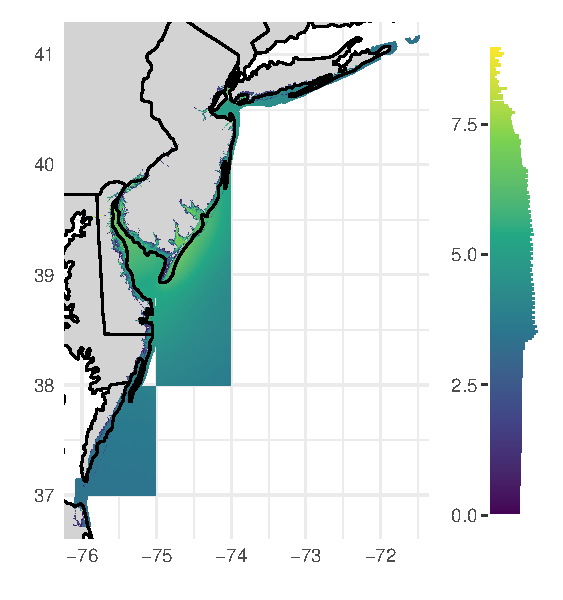
\includegraphics[width=0.99\linewidth]{./plots/slosh1run_loghist}
        \caption{Grid output from one storm simulation in SLOSH, with a marginal
            histogram (with log-scale counts) of surge levels in that storm 
            (truncated at 9 feet).\label{fig:slosh1run}\makenote{add boundaries to indicate
            range of directions and latitudes at which storm makes landfall.}}
    \end{subfigure}%
    ~ 
    \begin{subfigure}[t]{0.48\textwidth}
        \centering
        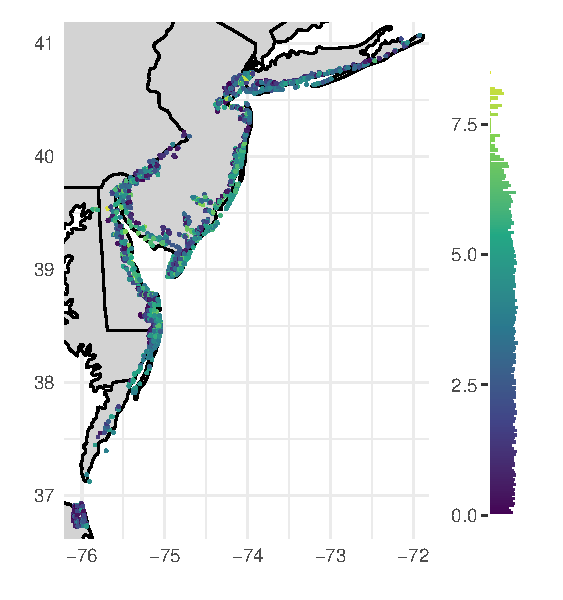
\includegraphics[width=0.99\linewidth]{./plots/sloshthreshold_loghist}
        \caption{
            90th percentile of storm-surge simulations at \num{5283} selected 
            locations with marginal histogram (with log-scale counts).
            \label{fig:sloshthreshold}}
    \end{subfigure}
    \caption{Exploration of SLOSH simulation data.\label{fig:sloshexplore}}
\end{figure}

This paper analyzes SLOSH simulations under an extreme value theory (EVT) framework, 
    using a peaks-over-threshold model.  EVT is a branch of statistics
    that focuses on the tails of the distribution---low density regimes where,
    in this application, the \emph{worst} outcomes occur.  
    We stress here a caveat. EVT assumes that the originating data are independent
    and identically distributed; SLOSH simulations do not meet the second criterion.
    They arise as a result of partially stochastic simulation given a set of input
    parameters---the storm characteristics.  Those storm characteristics themselves
    are sampled via Latin hypercube to fill the allowable parameter space.  That
    having been said, application of the EVT framework to SLOSH still provides us
    with a great deal of information.  It is with that caveat that we continue analysis.
    Figure~\ref{fig:sloshexplore} provides a visual depiction of the SLOSH 
    simulation data.  Figure~\ref{fig:slosh1run} indicates the output of a single 
    storm surge simulation using the SLOSH model. To the right of the map is a 
    histogram (with log-scale counts) displaying observed levels of inundation 
    in the storm, color-coded by the height of the surge at that location.  In this
    plot, there were 45 locations with surge greater than 9 feet above ground level,
    with the maximum value being approximately 19 feet above.  Such occurances
    are highly localized, and are not visible at this scale, so we truncated surge values
    in this plot at 9 feet.  We should also 
    note here that a storm takes some time to occur, and thus values recorded at 
    two locations in a single storm are not necessarily simultaneous.
    In Figure~\ref{fig:sloshthreshold}, we have selected SLOSH grid 
    cells that are in the vicinity of physical features, or locations, of 
    interest.  Displayed are the 90th percentile 
    of inundation for SLOSH simulations at each of those physical features.
    We make clear now, that this analysis is primarily concerned with the
    inferring and applying the dependence structure between storm surge at these locations,
    for storm simulations
    that are in excess of this threshold in at least one identified location.
    Our goal is then a consistent and performant model for multivariate extremes, 
    such that we can learn the dependence structure of extremes in the inundation field.
    \bruno{\bf This paragraph contains the right idea, but it needs to rewritten. Start
    by discussing the basic tenet of EVT is the ability to use a sample to infer how
    likely it is that the process will be over a certain value. You can say that it is
    straightforward to do this for each individual cell,  but complex dependencies 
    between cells is lost. Indicate that these are important in order to obtain joint 
    probabilities that two or more locations will have extreme behavior. A key information
    for the management of critical infrastructure. Throw in some references. Leave the
    issue of the sample not being really random to the end of the paragraph, yu don't
    want to start by being apologetic.}

\makenote{I need to expound upon the necessity/applicability of extreme analysis
    to inundation.  Mention: importance of tails of the distribution, relevance of
    extremes to such analysis, }

The paper proceeds as follows:  Section~\ref{ref:review} details the background 
    for the relevant modeling methods and dataset we will be using in this analysis.  
    In particular, Section~\ref{ref:evt} provides an overview of extreme value 
    theory, to the justification for separating the magnitude of a multivariate 
    extreme from its angular component; Section~\ref{ref:pg} describes the process 
    of creating an angular distribution as well as introducing the model we use in 
    our analysis; and Section~\ref{ref:varbayes} provides a brief review of variational
    inference which we attempt to use to speed analysis.  Section~\ref{slosh} further
    expands the discussion of the SLOSH dataset and how the analysis will proceed.
    Section~\ref{sec:methodology} expounds on the metrics we will be considering in
    our analysis as applications of the fitted angular model.  Further, 
    Section~\ref{ref:regression} introduces a novel regression model with support
    $\mathbb{S}_{p}^{d-1}$, the positive orthant of the $p$-norm unit sphere.
    Section~\ref{ref:results} presents our analysis, first evaluating the efficacy of
    variational methods on simulated data as compared to MCMC, then
    presenting some interesting results. Finally, Section~\ref{ref:conclusion} 
    concludes.

% EOF 